\documentclass[a4paper,11pt]{article}
% Created: 2008-7-1
\input{MyLayout.tex}
\usepackage{hologo}
\usepackage{xeCJK}
\setmainfont{Times New Roman}
\setCJKmainfont{FangSong}
\setCJKmonofont{FangSong}
\usepackage{setspace,amssymb,bbding,wasysym,eurosym,textcomp,graphicx,xpinyin}
\usepackage{fancyvrb}
\usepackage{picins}
\usepackage{color}
% 2008年7月13日20:42:06 标题中的``MetaPost'' 改成了 ``Asymptote''.
% MetaPost 断断续续看了好长时间还是稀里糊涂,
% 无意中发现了 Asymptote 比较合我的胃口,
% C++ 的语法看起来很熟悉,理解起来也容易多了。


\renewcommand{\figurename}{图}

\RecustomVerbatimEnvironment{Verbatim}{Verbatim}{%
frame=leftline, framerule=0.5mm, xleftmargin=2em,%
framesep=1mm, rulecolor=\color{red},%
baselinestretch=1, numbers=left, numbersep=1mm}

\definecolor{Mbackcolor}{RGB}{228,228,175}
\definecolor{Mzise}{RGB}{109,0,219}
\newcommand{\Memph}[1]{\textcolor{Mzise}{#1}}

\pagecolor{Mbackcolor}

\newcommand{\XeLaTeX}{\hologo{XeLaTeX}}



\begin{document}
\title{My \TeX{} \& Asymptote note}
\author{redspid@gmail.com}
\maketitle
\vspace{3cm}
\begin{center}
\begin{minipage}[t]{13cm}
{\Large ``[T]he \TeX{} research project that I embarked on was driven
by two major goals. The first goal was quality: we wanted to
produce documents that were
\Memph{not just nice, but actually the best.}''

``I never intended to have a system that would be universal and
used by everybody. I always wanted to write a system
that would be used for just the \Memph{finest} books.''

``The current version number for \TeX{} is $3.1$, and for METAFONT
it is $2.7$. If corrections are necessary, the next versions
of \TeX{} will be $3.14$, $3.141$, then $3.14159$, \ldots ,
converging to the ratio of a circle's circumference to its diameter;
for METAFONT the sequence will be $2.71$, $2.718$, . . . ,
converging to the base of natural logarithms. I intend to be fully
responsible for all changes to these systems for the rest of my life.''

\hfill Donald E. Knuth

\hfill {\it Digital Typography (1999)}}
\end{minipage}
\end{center}

\newpage
\tableofcontents
\listoffigures

\newpage
\section{什么是文件名数据库?怎样刷新?}
\TeX{} 系统通过这个数据库记录了所需要的各种文件的名字和具体目录位置。
每次向 \TeX{} 系统中添加文件后,都要记得刷新这个数据库,
否则 \TeX{} 有可能找不到需要的文件。

刷新文件名数据库的具体命令取决于当前的 \TeX{} 系统。
te\TeX{} 和 fp\TeX{} 的命令是:\Memph{texhash}

MiK\TeX{} 系统可以在命令行窗口输入 \verb+initexmf --update-fndb+

\section{如何安装宏包}
如果得到的宏包是已经编译过的,也就是已经有 \verb+.sty+ 或者 \verb+.cls+
文件,只需把这些文件放在 \verb+localtexmf\tex\latex\+ 下的某个子目录中,
可以自己建一个。然后还要让 \TeX{} 知道这个新的宏包的存在,
需要刷新 \TeX{} 系统的文件名数据库。现在你可以使用这个宏包了。

也可以把这些宏包文件和要编辑的 \TeX{} 源文件放在同一目录下,
这种情况下不需要刷新 \TeX{} 系统的文件名数据库,
但只有同一个目录下的文件可以使用这些宏包。

如果得到的是宏包的源文件,一般来说都包含两个文件:
一个扩展名为 \verb+.ins+ ,另一个扩展名为 \verb+.dtx+ 。
此外,通常会有一个 \verb+readme.txt+ 对宏包进行简要的说明。
现在需要两个步骤将它安装到 \TeX{} 系统中:
\subsection{生成样式文件并装入系统}
\begin{enumerate}
	\item 对 \verb+.ins+ 运行 \LaTeX{} 命令。
		这将会产生一个或若干个 \verb+.sty+ 文件
	\item 把 \verb+.sty+ 文件移到系统能找到的地方。
		通常是 \verb+.../localtexmf/tex/latex+
		子目录下(Windows 或者 OS/2 用户应该改变斜线为反斜线)
	\item 刷新系统的文件名数据库。参照上一节的说明
\end{enumerate}

\subsection{生成说明文档}
\begin{enumerate}
	\item 对 \verb+.dtx+ 文件运行 \LaTeX{} 命令。
		这将会产生一个 \verb+.dvi+ 文件。
		注意:可能需要多次运行 \LaTeX{} 来正确处理交叉引用
	\item 检查一下 \LaTeX{} 是否产生了 \verb+.dvi+ 文件。
		如果没有发现这个文件,就可以执行第 5 步了。
	\item 为了生成索引,键入命令:\verb+makeindex -s gind.ins name+
		(这里 name 表示不带扩展名的主文件名)
	\item 再次对  \verb+.dtx+ 文件运行 \LaTeX{} 命令。
	\item 最后一步不是必需的,生成 \verb+.ps+ 文件或者 \verb+.pdf+
		文件以方便阅读。
\end{enumerate}
有时会发现生成了一个 \verb+.glo(glossary)+ 文件。
在第 4 步和第 5 步之间运行下面的命令
\begin{Verbatim}
makeindex -s gglo.ist -o name.gls name.glo
\end{Verbatim}
确认在执行第 5 步前最后对 \verb+.dtx+ 文件运行一遍 \LaTeX{} 命令。

\section{建立自己的包}
如果建立了很多自己的环境和命令,文档导言部分将变得很长,
在这种情况下,建立一个新的 \LaTeX{} 包来存放所有自定义的命令和环境是一个%
好的处理方式。可以在文档中使用 \verb+\usepackage+ 命令来引入中定义宏包%
中的环境和命令。

写一个宏包的基本工作就是将文档导言复制到一个分离的文件中去,
这个文件要以 \verb+.sty+ 结尾。还需要一个命令:
\begin{Verbatim}
\ProvidesPackage{package_name}
\end{Verbatim}

这个命令应该在包定义源文件的最前面使用。它用于告诉 \LaTeX{} 宏包的名称%
从而允许 \LaTeX{} 在你尝试两次引入同一个宏包的时候给出一个良好的错误信息。

\section{在 CJK 中如何调整汉字的间距}
CJK 会在两个汉字间插入一个 \verb+\CJKglue+,
因此我们修改 \verb+\CJKglue+ 的定义就可以调整汉字的间距:
\verb+\renewcommand{CJKglue}{\hskip<b>plus<p>minus<m>}+\\
其中\verb+<b>+、\verb+<p>+和\verb+<m>+都是 \TeX{} 长度,如 $0.05pt$。
执行以上命令后,汉字的标准间距就是\verb+<b>+,在需要的时候可以增加或减少,
调整幅度分别不超过\verb+<p>+和\verb+<m>+。

CJK 的默认值是 \verb+\hskip 0pt plus 0.08\baselineskip+ 。

CJK环境中改字体命令: \verb+\CJKfamily{fontName}+

\section{首段缩进 和 段首缩进}
\verb+\usepackage{indentfirst}+ 宏包可指定首段缩进。

article 文档类默认首段缩进 2em ,从正文看可能比两个字符的宽度小一点,
因为两个字符间有个间距,可在导言区用 \verb+\parindent+ 指令自定义段首缩进。

\section{\LaTeX{}-Suite 安装}
\subsection{GNU/Linux、Unix类}
\begin{spacing}{1}
\begin{enumerate}
	\item 创建 \verb+~/.vimrc/+ 目录
	\item 将 \LaTeX{}-Suite 压缩包中内容复制到其中
	\item 在 \verb+~/.vimrc/.vimrc+ 中添加下面代码(引号开头的是注释行,
		可以删除,建议保留)\\
		{\footnotesize
		\begin{verbatim}
		" ------------begin latex-suite ---------------
		" REQUIRED. This makes vim invoke latex-suite when you open a tex file.
		" filetype plugin on

		" let vim invoke latex-suite when you a file which has postfix .tex
		let g:tex_flavor="tex"

		" IMPORTANT: win32 users will need to have 'shellslash' set so that latex
		" can be called correctly.
		set shellslash

		" IMPORTANT: grep will sometimes skip displaying the file name if you
		" search in a singe file. This will confuse latex-suite. Set your grep
		" program to alway generate a file-name.
		set grepprg=grep\ -nH\ $*

		" OPTIONAL: This enables automatic indentation as you type
		filetype indent on
		" ------------ end latex-suite ------------
		\end{verbatim}}
\end{enumerate}
\end{spacing}

\subsection{Windows}
\begin{enumerate}
	\item 将 \LaTeX{}-Suite 压缩包中内容复制到 \verb+...\vim\vimfiles\+ 中
	\item 在 \verb+...\vim\_vimrc\+ 中添加代码(与上小节相同)
\end{enumerate}

\LaTeX{}-Suite 中给出的配置文件预设状态是让 Vim
以打开文件的内容来判断是否 \TeX{} 文件(上面的代码我已做了修改,
以文件名判断打开文件的类型),若是,则调用 \LaTeX{}-Suite。

\section{字体相对大小}
当前 normalsize 大小为 12pt 。\\
{\tiny tiny} {\scriptsize scriptsize} {\footnotesize footnotesize}
{\small small}
normalsize {\large large} {\Large Large} {\LARGE LARGE}
{\huge huge} {\Huge Huge}

\section{指定字号}
\verb+\fontsize{size}{baselineskip}\selectfont+ 第一个参数指定字号,
第二个参数指定 baselineskip,然后\verb+\selectfont+命令执行选定的字体。

例:\verb+\fontsize{36}{38}\selectfont+
{\fontsize{36}{38}\selectfont 三十六号字}

\section{\LaTeX{} 画线}
\verb+\rule[lift]{width}{height}+

\section{纸张尺寸设置}
\verb+\paperheight=26cm+\\
\verb+\paperwidth=20cm+\\

注意当前的 \verb+\textheight+ 和 \verb+\textwidth+ 设置,
应在纸张大小的范围内。

\subsection{对于dvips}
导言区加入: \verb+\special{papersize=<width,heith>}+

\subsection{对于pdftex / pdflatex}
导言区加入: 
\begin{Verbatim}
\setlength{\pdfpageheight}{<height>} 
\setlength{\pdfpagewidth}{<width>} 
\end{Verbatim}

\subsection{对于 dvipdfm(x)}
导言区加入: \verb+\special{pdf: pagesize width <width> height <height>}+


\section{图形和表格目录}
\verb+\listoffigures+ 指令排版图形目录,\verb+\listfigurename+
为图形目录标题。\\
\verb+\listoftables+ 指令排版表格目录,\verb+\listtablename+
为表格目录标题。

\section{图文混排}
\subsection{wrapfig 宏包}
用法:%
\verb+\begin{wrapfigure}{行数}[位置][超出长度]{宽度}<图形>\end{wrapfigure}+\\
行数是指图形高度所占的文本行的数目。 如果不给出此选项,
wrapfig 会自动计算。 位置是指图形相对于文本的位置,须给定下面四项的一个。
\begin{itemize}
	\item {\bf r,R} 表示图形位于文本的右边
	\item {\bf l,L} 表示图形位于文本的左边
	\item {\bf i,I} 表示图形位于页面靠里的一边(用在双面格式里)
	\item {\bf o,O} 表示图形位于页面靠外的一边
\end{itemize}
超出长度是指图形超出文本边界的长度,缺省为 $0pt$。 宽度则指图形的宽度。
wrapfig 会自动计算图形的高度。不过,我们也可设定图形的高度,
具体可见 wrapfig.sty 内的说明。

例:
\begin{Verbatim}
\usepackage{graphicx}
\usepackage{wrapfig}
...
\begin{wrapfigure}{r}{4.5cm}
\includegraphics [width=4cm,clip]{yourfigure.pdf}
\end{wrapfigure}
\end{Verbatim}

\subsection{picins 宏包}
texlive2017 未包含 picins 宏包。
下载,解压后将 picins 目录复制到 \verb+texlive/texmf-local/tex+ 目录下。
运行 \verb+texhash+ 更新文件名数据库即可。

用法:%
\verb+\parpic(宽度,高度)(水平偏移,垂直偏移)[选项][位置]{图形}+

{\bf 位置}只能为下面两个中的一个
\begin{itemize}
	\item [l] 将图形置于文本段落的左方(这也是缺省值)
	\item [r] 将图形置于文本段落的右方
\end{itemize}

{\bf 外观}只能为下面五个中的一个,可与上述位置项配合使用
\begin{itemize}
	\item [f] 将图形置于一个实框盒子中
	\item [d] 将图形置于一个虚框盒子中
	\item [o] 将图形置于一个圆角框盒子中
	\item [s] 将图形置于一个具有阴影效果的盒子中
	\item [x] 将图形置于一个具有立体效果的盒子中	
\end{itemize}

{\bf 位置}仅当给定的宽度和高度与图形的实际大小相差很大的情况下才起作用。
若税票活垂直偏移已给出,那么此项也不起作用。
缺省位置是将图形置于盒子的中央。也可以取以下的值:
\begin{itemize}
	\item [l] 将图形置盒子的左方
	\item [r] 将图形置于盒子的右方
	\item [t] 将图形置于盒子的上方
	\item [b] 将图形置于盒子的下方
	\item [x] 将图形置于一个具有立体效果的盒子中	
\end{itemize}
例如图\ref{arrow_show} ``Asymptote 指示箭头'' 一节中使用的插图代码:\\
\verb+\parpic[r]{\includegraphics[scale=0.7]{arrow_show.pdf}}+

用下面的代码为混排的图片增加 caption 和 label :
\begin{Verbatim}
\piccaption{yourcaption\label{yourlabel}}
\parpic[r]{\includegraphics{show.pdf}}
\end{Verbatim}

可在 \verb+\parpic+ 指令后面的小括号内设置图片所占空间大小%
(必须宽、高同时设定,不能缺项。这里不是图片大小,
图片大小用\verb+\includegraphics+的 width 参数设定)。
插入图\ref{string_label}的代码如下:
\begin{Verbatim}
\piccaption{Asymptote 文字外框\label{string_label}}
\parpic(5cm,3cm)[r]{\includegraphics{string_label.pdf}}
\end{Verbatim}

\section{堆叠符号}
用\verb+\stackrel{}{}+可将两个符号竖直堆叠起来。\\
例如:\verb|$\stackrel{y\to+\infty}{x\to+\infty}$|
的效果:$\stackrel{y\to +\infty}{x\to +\infty}$

若要以相同大小堆叠,可用\verb+\atop{}+命令。\\
例如:\verb|$y\to +\infty\atop{x\to +\infty}$|
的效果:$y\to +\infty\atop{x\to +\infty}$

\section{分隔符$\mid$}
\verb+$\{x\mid x>0\}$+$\quad\{x\mid x>0\}$

\section{存储盒子的用法}
\begin{Verbatim}
\newsavebox{\mybox}    %定义盒子名称
\savebox{\mybox}{测试存储盒子的用法}  %定义盒子内容

\usebox{\mybox}  %使用盒子,出现的将是盒子内容
\end{Verbatim}
定义盒子的完整形式为:\verb+\savebox{\boxname}[width][pos]{...}+

\section{文字、背景颜色}
彩色文字和背景需导入 \Memph{color} 宏包:\verb+\usepackage{color}+ ,
中文环境需将这条指令置于 \verb+\begin{CJK}+ 下面。\\
例:\verb+\textcolor{red}{红色的文字}+:\textcolor{red}{红色的文字}

\section{\XeLaTeX}
三天前(2017-06-09)开始用 \XeLaTeX ,把一堆问题折腾好了,
当我写这段笔记的时候,哇哦\ldots 竟然发现打不出 \XeLaTeX 符号,
编译器提示\verb+\XeLaTeX+这个宏 undefined.

搜了一圈没搜到,暂时用 \verb+Xe\LaTeX+ 替代。
先自己定义一下吧 \verb+\newcommand{\XeLaTeX}{Xe\LaTeX}+,
等找到了直接删除 newcommand 定义。

源文件全部使用 utf-8 编码。中文使用 xeCJK 宏包。

\XeLaTeX 最大的好处是可以方便地用\verb+\CJKfontspec{}+来变更中文字体了。

{\CJKfontspec{LiSu}(隶书)看这里!}
{\CJKfontspec{YouYuan}(幼圆)看这里!}
{\CJKfontspec{STXingkai}(华文行楷)看这里!}

还是尽量选择通用的字体,兼容不同的编译环境。还要注意字体的授权问题。

中文等宽字体还是需要设置的,复杂的文档一般会用到,不设置编译器会报错。
\verb+\setCJKmonofont+

现在觉得宏包的详细用法没必要写笔记,还是看宏包文档方便。
这里就留着记录一下 \XeLaTeX 这个坑。

(2017-06-12 15:15:26)
OK,现在可以把上午挖的坑填上了。在知乎上提了问题,得到了解答。

默认确实没有定义 \verb+\XeLaTeX+ , hologo 宏包里面提供了这些logo。
现在本文引入了 hologo 宏包,\XeLaTeX 的定义改成了:
\verb+\newcommand{\XeLaTeX}{\hologo{XeLaTeX}}+

\section{拼音宏包 xpinyin}
原来用 pinyin+ruby 宏包写拼音,因为宏包兼容问题,还没法合并到这个文档。
发现了 xpinyin 更好用,不但能自动注音,其它功能也丰富得多。

简单记一下常用命令:
\begin{itemize}
	\item \verb+\pinyin{pin1yin1}+ 输出拼音
	\item \verb+\xpinyin{音}{yin1}+ 给单个汉字手工注音
	\item \verb+\xpinyin*{拼音}+ 给汉字自动注音
	\item \verb+pinyinscope+ 自动注音环境。
\end{itemize}

\verb+xpinyinsetup{key=value}+ 设置选项。\verb+multiple={\color{red}}+
可以自动将多音字的注音显示为红色,需要引入 color 宏包。

\vspace{3mm}
示例: {\LARGE\xpinyin*[multiple={\color{red}}]{车如流水马如龙,花月正春风}}


\section{Asymptote 指示箭头}
\piccaption{Asymptote 指示箭头演示图\label{arrow_show}}
\parpic[r]{\includegraphics[scale=0.7]{./figs/arrow_show.pdf}}
\begin{Verbatim}
size(10cm,0);
texpreamble("\usepackage{amsmath}");

path p = (0,0)..(1,1)..(2,.5){dir(0)};
real al  = arclength(p);
real l   = length(p);
pair pt  = point(p,l/2);
pair apt = arcpoint(p,al/2);

draw(p);
draw(subpath(p,0,arctime(p,al/2)),blue);

// 指向 pt 的箭头,文字位于 pt 的 SSE,箭头长度 1cm
dot(pt,red); dot(apt,blue); 

// 指向 pt 的箭头,文字位于 apt 的 SSW,箭头长度 1cm
arrow("$\frac{\text{lenght(p)}}{2}$",pt,SSE,1cm);
arrow("$\frac{\text{arclenght(p)}}{2}$",apt,SSW,1cm);
label("\small The sizes of the blue path and the black path are equal",
      (1,.25));
\end{Verbatim}

\section{用 \LaTeX -Suite 导入模板}
安装 LaTeX{}-Suite 后可以用 \Memph{:TTemplate} 命令列出已有的模板列表。%
也可以用 \mbox{\Memph{:TTemplate tname}} 导入名为 \Memph{tname} 的模板。
\Memph{:TTemplate} 可按照 \TeX{} 规则简写为 \Memph{:TTe} 。

(2008-7-22 12:15:21)模板导入时会自动缩进,可能导致格式错乱。
现在我在 \_vimrc 中加入两个自动命令来解决:
\begin{Verbatim}
autocmd BufReadPre
filetype indent off
autocmd BufReadPost
filetype indent on
\end{Verbatim}
这个方法在引入较复杂的,例如有 \Memph{tabular} 环境的模板时仍会出现自动缩进的问题。

\section{Asymptote 带边框的文字}
\piccaption{Asymptote 文字外框\label{string_label}}
\parpic(5cm,3cm)[r]{\includegraphics{./figs/string_label.pdf}}
\verb+point(object, -1)+为对象左连接点,
\verb+point(object, 1)+为对象右连接点。
\begin{Verbatim}
currentpen = linewidth(2bp);

// draw(string, path, pair, 文字与边界的margin);
object hello = draw("Hello", box, (0,15mm),1mm);
object world = draw("World", ellipse, (0,0), 2mm);

draw(point(hello, -1){SW} .. {W}point(world, 1), Arrow(TeXHead));
\end{Verbatim}

\section{Asymptote labelpath}
这个模块使用 PSTricks pstextpath 宏使 labels 按照一个 path 排列%
(像示例文件 curvedlabel.asy 中一样适当紧密排列)。

\begin{Verbatim}
函数原型:
void labelpath(picture pic=currentpicture, Label L, path g,
               string justify=Centered, pen p=currentpen);
\end{Verbatim}

这里 justify 是 LeftJustified、Centered 或 RightJustified 其中的一个。
The x component of a shift transform applied to the Label is
interpreted as a shift along the curve, whereas Chapter 7: Base
modules 91 the y component is interpreted as a shift away from the curve.
All other Label transforms are ignored. This package requires
the latex tex engine and inherits the limitations of the
PSTricks \verb+\pstextpath+ macro.
\piccaption{labelpath 示例\label{label_path}}
\parpic[r]{
\includegraphics{./figs/label_path.pdf}}

Note: 源码文件命名的时候不能与代码中导入的 module 同名,
否则可能被编译器认为是递归调用 module 。

图\ref{label_path}代码如下:
\begin{Verbatim}
size(4cm, 0);
import labelpath;

labelpath("This is a test of curved labels
           in Asymptote.",
          reverse(rotate(-90)*unitcircle));
\end{Verbatim}

Note: labelpath 中的文字需要用 tex 命令来编译,不能用 pdflatex,
在使用 CTeX 软件包时就会因中文字体问题导致字符显示不出来。

\section{\LaTeX -Suite hotkey}
\begin{itemize}
\item \verb+<F5>+键可自动扩展当前 word 为环境模式(在正文部分),
在导言部分可扩展当前 word 为\verb+\usepackage{word}+
\item \verb+<F7>+键可自动扩展当前 word 为命令模式
\item 和环境扩展以`E' 开通类似,字体环境以`F'开头。
	`FEM'即扩展为: \verb|\emph{}<++>|
\item ALT-l 键扩展为:\verb|\label{}<++>|
\end{itemize}

\subsection{智能扩展字符:}
\begin{Verbatim}
'__' -> '_{<++>}<++>'                 '()' -> '(<++>)<++>'
'[]' -> '[<++>]<++>'                  '{}' -> '{<++>}<++>'
'^^' -> '^{<++>}<++>'                 '$$' -> '$<++>$<++>'
'==' -> '&=& '                        '~~' -> '&\approx& '
'=~' -> '\approx'                     '::' -> '\dots'
'((' -> '\left( <++> \right)<++>'
'[[' -> '\left[ <++> \right]<++>'
'{{' -> '\left\{ <++> \right\}<++>'
\end{Verbatim}

\subsection{重复键入自动扩展字符}
\begin{Verbatim}
= -> \equiv                            \\ -> \setminus
'.' -> \cdot                           '*' -> \times
'&' -> \wedge                          '-' -> \bigcap
'+' -> \bigcup                         'M' -> \sum_{<++>}^{<++>}<++>
'S' -> \sum_{<++>}^{<++>}<++>          '(' -> \subset
')' -> \supset                         '<' -> \le
'>' -> \ge                             ',' -> \nonumber
'~' -> \tilde{<++>}<++>                ';' -> \dot{<++>}<++>
':' -> \ddot{<++>}<++>
\end{Verbatim}

\subsection{$\backprime$前缀扩展字符:}
\begin{Verbatim}
^ -> \hat{<++>}<++>                    _ -> \bar{<++>}<++>
6 -> \partial                          8 -> \infty
/ -> \frac{<++>}{<++>}<++>             % -> \frac{<++>}{<++>}<++>
@ -> \circ                             0 -> ^\circ
2 -> \sqrt{<++>}<++>                   | -> \Big|
I -> \\int_{<++>}^{<++>}<++>
\end{Verbatim}

\subsection{希腊字母:}
\begin{Verbatim}
a -> \alpha              b -> \beta              c -> \chi
d -> \delta              e -> \varepsilon        f -> \varphi
g -> \gamma              h -> \eta               k -> \kappa
l -> \lambda             m -> \mu                n -> \nu
p -> \pi                 q -> \theta             r -> \rho
s -> \sigma              t -> \tau               u -> \upsilon
v -> \varsigma           w -> \wedge             x -> \xi
y -> \psi                z -> \zeta
\end{Verbatim}
{\huge\textcolor{red}{\makebox[\textwidth][s]{
$\alpha{}\ \beta{}\ \chi{}\ \delta{}\ \varepsilon{}\ %
\varphi{}\ \gamma{}\ \eta{}\ \kappa{}\ \lambda{}\ \mu{}\ \nu{}\ %
\pi{}\ \theta{}\ \rho{}\ \sigma{}\ \tau{}\ \upsilon{}\ %
\varsigma{}\ \wedge{}\ \xi{}\ \psi{}\ \zeta$}}}

不是所有的希腊字母在 \LaTeX -Suite 中都有大写形式,\\
可参考 \verb+http://www.giss.nasa.gov/latex/ltx-405.html+
\begin{Verbatim}
D -> \Delta              G -> \Gamma             F -> \Phi
L -> \Lambda             X -> \Xi                Q -> \Theta
Y -> \Psi                S -> \Sigma             U -> \Upsilon
W -> \Omega
\end{Verbatim}
{\huge\makebox[0.7\textwidth][s]{\textcolor{red}{
$\Delta{}\ \Gamma{}\ \Phi{}\ \Lambda{}\ \Xi{}\ \Theta{}\ \Psi{}\ %
\Sigma{}\ \Upsilon{}\ \Omega$}}}

\section{Asymptote: 轴对称变换}
\piccaption{轴对称变换\label{asy_reflect}}
\parpic[r]{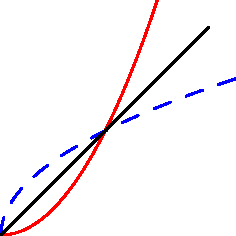
\includegraphics{./figs/reflect.pdf}}
\begin{Verbatim}
size(4cm);
import graph;
pen drawpen = linewidth(bp);

real f(real t) { return t^2; }
path ff = graph(f, 0, 1.5, operator..);
draw(ff, drawpen+red);

draw(reflect((0,0),(1,1)) * ff, drawpen+blue+dashed);

draw((0,0)--(2,2), drawpen);
\end{Verbatim}

\section{Asymptote: 标记角度}
使用 \Memph{markers} 包中的 \Memph{markangle()} 函数为角度做标记。
\verb+\angle+$\to \angle$ 。

\vspace{4mm}
函数原型:
\piccaption{标记角度\label{asy_angle}}
\parpic[r]{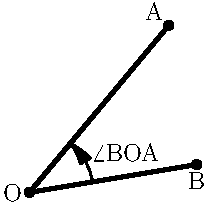
\includegraphics{./figs/angle.pdf}}
\begin{Verbatim}
void markangle(picture pic=currentpicture, Label L="",
               int n=1, real radius=0, real space=0,
               pair A, pair O, pair B, arrowbar arrow=None,
               pen p=currentpen, margin margin=NoMargin,
               marker marker=nomarker);
\end{Verbatim}

示例(图\ref{asy_angle}):
\begin{Verbatim}
import markers;
pair A=(50,60), B=(60,10), origin=(0,0);
draw(A--origin--B, linewidth(2bp));
markangle("\angle BOA", B, origin, A, Arrow, linewidth(bp));
\end{Verbatim}

\section{Asymptote 中的中文}
Asymptote 使用 \TeX{} 处理中文,
按图\ref{asy_chinese}中这样在生成的图像中使用中文:
\piccaption{在 Asymptote 中使用中文\label{asy_chinese}}
\parpic(5.5cm,3cm)[r]{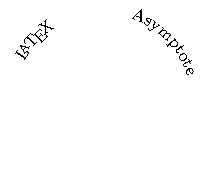
\includegraphics{./figs/chinese.pdf}}
\begin{Verbatim}
import labelpath;
size(100);
texpreamble("\usepackage{CJK}\AtBeginDocument{
            \begin{CJK}{GBK}{fs}}
            \AtEndDocument{\clearpage\end{CJK}}");
labelpath("\scriptsize 现在可以像在 \LaTeX{}
          中一样在 Asymptote 中使用中文",
          reverse(rotate(-90)*unitcircle));
\end{Verbatim}

在源文件头加入设定: \verb+settings.tex=pdflatex+ 可以指定用 pdflatex
命令编译 label,并直接生成 PDF 的图形,避免默认的编译器造成缺少汉字%
字体的问题。

Note: labelpath 中的文字需要用 tex 命令来编译,不能用 pdflatex,
在使用 CTeX 软件包时就会因中文字体问题导致字符显示不出来。
所以仅在不使用 labelpath,只使用 label 的时候用 pdflatex 编译。

\section{Asymptote 的线条连接风格}
\piccaption{linecap(0、1、2) 三种连接风格\label{connection_style}}
\parpic(7cm,2cm)[r]{
\includegraphics{./figs/connection_style.pdf}}
\begin{Verbatim}
pen squarecap = linecap(0);
pen roundcap = linecap(1);
pen extendcap = linecap(2);
\end{Verbatim}

\section{Asymptote: 导入图像文件}
\verb+string graphic(string name, string options="")+\\
返回一个可以用来导入 EPS 文件的 string 变量(只能导入 EPS 格式文件)。

这里 \Memph{name} 是被导入的 EPS 文件名。
\Memph{option} 是一个包含下面选项的用逗号分割的参数列表。
\begin{itemize}
\piccaption{Asymptote 导入图像文件\label{input_fig}}
\parpic(6cm,4.5cm)[r]{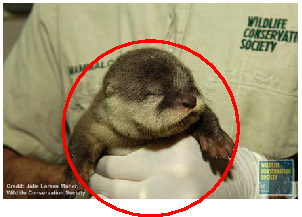
\includegraphics{./figs/input_fig.pdf}}
	\item (bb=llx lly urx ury) bounding box
	\item (width=value) width
	\item (height=value) height
	\item (angle=value) rotation
	\item (scale=factor) scaling
	\item (clip=bool) clipping
	\item (draft=bool) draft mode
\end{itemize}

\Memph{void layer()} 函数可以将后面添加的对象放在导入的图像上层。

图\ref{input_fig}的代码:
\begin{Verbatim}
label(graphic("hb.eps", "width=5cm, clip=true"),
      position=(0,0));
layer();
draw(circle((0,-13), 42), linewidth(bp)+red);
\end{Verbatim}

%The string baseline(string s, align align=S, string template="M")
%function can be used to enlarge the bounding box of letters
%aligned below a horizontal line to match a given template,
%so that their baselines lie on a horizontal line.
%See Pythagoras.asy for an example.
%

\section{\LaTeX{} 中局部行距设置}
可用 \Memph{setspace} 宏包设置局部行距。如下所示:
\begin{Verbatim}
\usepackage{setspace}
\begin{spacing}{1.8}
.....................
\end{spacing}
\end{Verbatim}

\section{Asymptote: cut() 和 struct slice}
\verb+slice cut(path p, path knife, int n);+\\
以 \verb+struct slice { path before,after; }+ 形式返回路径 p
被与路径 knife 第 n(\Memph{从$0$开始计数}) 个交点分隔开的前、
后两部分(如果两条路径没有交点,整个路径 p 都被认为是交点`前'的部分)。

参数 n 会对交点数取模($n \% numOfIntersection$)。

\verb+slice firstcut(path p, path knife);+
等价于 \verb+cut(p, knife, 0);+ 。

\verb+slice lastcut(path p, path knife);+
等价于 \verb+cut(p, knife, -1);+ 。
\piccaption{cut 函数和 sturct slice 示例\label{cut_slice}}
\parpic(7cm, 3cm)[r]{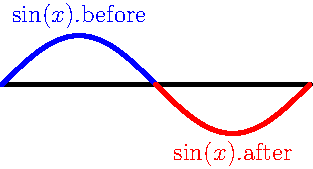
\includegraphics{./figs/cut_slice.pdf}}
示例代码(图\ref{cut_slice}):
\begin{Verbatim}
size(150); import graph; defaultpen(2bp);

path s = graph(sin, 0, 2pi);
path h = (0,0) -- (6.3,0);
draw(h);

slice k = cut(s, h, 1);
draw("$sin(x)$.before", k.before, N, blue);
draw("$sin(x)$.after", k.after, S, red);
\end{Verbatim}

\section{Asymptote 颜色名称}
\begin{figure}[htpb]
\centering
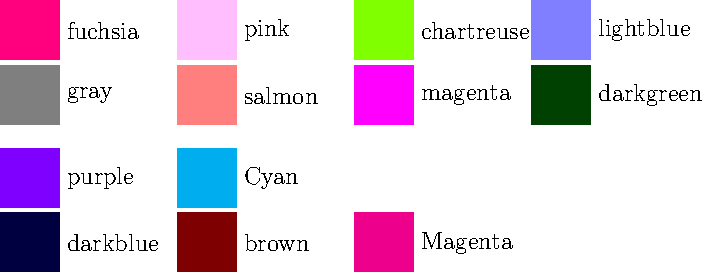
\includegraphics[scale=0.7]{./figs/asy_color.pdf}
\caption{Asymptote 颜色名称}
\label{fig:asy_color}
\end{figure}

颜色由深到浅的修饰词: dark$\to$deep$\to$heavy$\to$*$\to$medium$\to$light%
$\to$pale 。

如图\ref{fig:asy_color2}所示:
\begin{figure}[htpb]
\centering
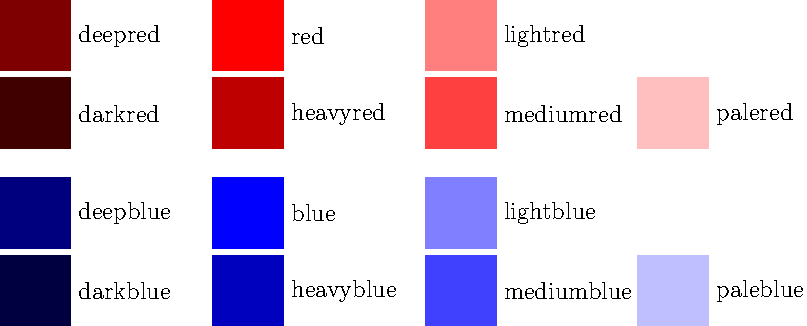
\includegraphics[scale=0.7]{./figs/asy_color2.pdf}
\caption{颜色由深到浅的修饰词}
\label{fig:asy_color2}
\end{figure}

\section{Asymptote: 字体大小,Arrow、UnFill 大小 和 xtick}
下面代码第 3行设置定义默认字体大小,
也可用\verb+defaultpen(fontsize(12pt))+形式。

第 14、15行代码方位标志\Memph{S}前的数字表示
label 与标记点的距离,
\verb+UnFill(real)+中参数定义空白大小(\Memph{Note:}不是dot大小,
dot大小由linewidth() 或 dotfactor 设定)。

图\ref{dot_label_tick}的 $a$标记点周围有空白,
这就是\verb+UnFill(real)+的设置过大。

\piccaption{字体.Arrow.UnFill\\大小设置\label{dot_label_tick}}
\parpic[r]{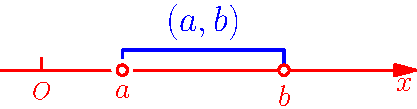
\includegraphics[width=0.4\textwidth]{./figs/dot_label_tick.pdf}}
\begin{Verbatim}
import graph;
size(200,0);
defaultpen(1bp+red); //设定默认pen直径和颜色
defaultpen(fontcommand("\large"));

xlimits(0,10);
xaxis("$x$", Arrow(10pt)); //Arrow(real) 中参数可以设定大小
xtick("$O$", 1); //第二个参数也可以用 pair
pair a=(3,0), b=(7,0), rise=(0,0.5);

draw("$(a, b)$", a--(a+rise)--(b+rise)--b,
    N, blue+fontsize(16pt));//最后一个参数定义此处的pen和字体大小

dot("$a$", a, 2S, UnFill(3pt));
dot("$b$", b, 2S, UnFill);
\end{Verbatim}

\section{Asymptote: size()函数}
size(200); //x=200,y=200\\
size(200,0); //x=200, y不限制\\
size(0,200); //x不限制, y=200\\
size(0,0); //直接采用 PostScript 的坐标,最终不做任何图形尺寸的控制,
这时作图等价于 MetaPost 的手工控制最终图形的尺寸。

\section{特殊符号}
宏包导入太多命令会冲突,ifsym\footnote{导入天气符号需要用 weather 选项}%
里面有好多漂亮的符号就没法在这里 show 了,
我找找有没有导入局部命令的方法\footnote{似乎目前还没有好的办法%
可以完美解决这个问题,关于汉字注音的笔记由于和希腊字母命令冲突,
只能放在 addtional.tex 里面了}。特殊符号参考文档 symbols 。
\Memph{bbding} 宏包一定要在 \Memph{wasysym} 之前导入:\verb+\usepackage{bbding, wasysym}+

\begin{tabular}[hbtp]{ccl|ccl}
\permil & wasysym & \verb+\permil+ & \HandLeft & bbding & \verb+\HandLeft+\\
\HandRight & bbding & \verb+\HandRright+ & \HandLeftUp & bbding & \verb+\HandLeftUp+\\
\HandRightUp & bbding & \verb+\HandRightUp+ & \HandPencilLeft & bbding & \verb+\HandPencilLeft+\\
\Peace & bbding & \verb+\Peace+ & \Phone & bbding & \verb+\Phone+\\
\PhoneHandset & bbding & \verb+\PhoneHandset+ & \Envelope & bbding & \verb+\Envelope+\\
\Plane & bbding & \verb+\Plane+ & \Tape & bbding & \verb+\Tape+
\end{tabular}

\subsection{带外圈的符号}
\verb+\textcircled{A}+ \textcircled{A}

汉字比英文字母大一点会跑到圈外面:\verb+\textcircled{字}+ \textcircled{字}

\subsection{货币符号}
\verb+\$+ \$\hspace{1cm}\verb+\pounds+ \pounds

textcomp 宏包:
\verb+\textcent+ \textcent\hfill
\verb+\textyen+ \textyen\hfill
\verb+\textsterling+ \textsterling

eurosym 宏包:
\verb+\geneuro+ \geneuro\hfill
\verb+\geneuronarrow+ \geneuronarrow\hfill
\verb+\geneurowide+ \geneurowide\hfill
\verb+\officialeuro+ \officialeuro

\section{Beamer 文档类}
\begin{itemize}
	\item 在\verb+\section{}+参数中用汉字,
		需在导入 beamer 文档类时加 CJK 参数:\\
		\verb+\documentclass[CJK]{beamer}+
	\item \verb+\begin{CJK}{GBK}{fs}+要放在 \verb+\begin{document}+ 下面。
	\item 需使用\verb+\verb+命令或 verbatim 环境的 frame 要带参数
		\Memph{fragile}:\verb+\begin{frame}[fragile]+\\
			并且此时不可直接在 frame 环境参数中写 \Memph{frametitle},
			而应用 \verb+\frametitle{}+ 命令。
	\item 导言区加入\verb+\setbeamertemplate{navigation symbols}{}+
		取消导航条。
	\item \verb+\includegraphics[]{}+定义宽度或高度参数需明确写:
		``[width=]'' 或 ``[height=]'' 。
\end{itemize}

\section{自定义颜色}
使用 \Memph{color} 宏包的 \verb+\definecolor{name}{mode}{color-spec}+
命令可以自定义颜色。这个笔记中 \Memph{强调文本}
的颜色就是用下面的代码定义的:
\begin{Verbatim}
	\definecolor{Mzise}{RGB}{109,0,219}
	\newcommand{\Memph}[1]{\textcolor{Mzise}{#1}}
\end{Verbatim}

除了用 \Memph{RGB} 模式定义颜色外,还可以用 \Memph{cmyk} 或其它模式,
目前 RGB 颜色已经够用了。

\section{单/双栏混排}
\Memph{cuted}宏包用于在双栏选项下提供 Full width 的单栏环境。
\begin{Verbatim}
\documentclass[a4paper,twocolumn,10pt]{article}
\usepackage{cuted}
\begin{document}
% 此处为双栏...
\begin{strip}
	% 此处单栏...
\end{strip}
\end{document}
\end{Verbatim}


\section{Asymptote: 多行文本的 label}
需要在图中使用多行文本,可以用 minipage 函数:
\piccaption{Asymptote 导入图像文件\label{label_muti_lines}}
\parpic(4.3cm,4.3cm)[r]{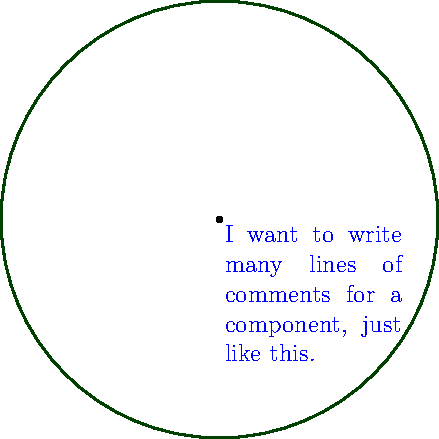
\includegraphics[width=3.9cm]{./figs/label_muti_lines.pdf}}
\begin{Verbatim}
pair O=(0,0);
string l = "I want to write many lines of comments
	for a component, just like this.";
draw( circle(O, 37mm), 1bp+darkgreen );
dot(O);
label( minipage(l, 30mm), (0,0), SE, blue);
\end{Verbatim}

\section{Asymptote: settings}
Asymptote 的设定项:
\begin{itemize}
	\item settings.outformat="pdf\verb+|+png\verb+|+jpg\ldots" 设定图形格式
	\item settings.tex="xelatex" 指定 label 的编译器
\end{itemize}

Asymptote 使用 ghostscript 生成 PDF 格式文件,因此,
需要先安装 ghostscript 。

\section{Asymptote: 分页输出}
\verb+shipout("FileNamePrefix")+

\section{Asymptote: tips}
\subsection{变量名冲突}
变量名冲突: E S W N,是预定义变量,避免作为自定义变量使用。

\subsection{语法}
Transform 顺序:  \verb+transform * Lable;+

\subsection{pair 赋值默认行为}
对 pair 变量赋值时,若直接用一个数字,则 y 坐标默认为0 。
\begin{Verbatim}
pair origin = 0;    // origin = (0,0)
pair A = 7;    // A = (7,0)
\end{Verbatim}

\subsection{颜色计算}
颜色可以与 real 相乘, $real\in [0,1]$ ,乘以$0$是黑色,乘以$1$是本色。
\begin{Verbatim}
0.5*red;
0.9*yellow;
\end{Verbatim}


\section{在宏包中使用 CJK 包\Mdepr}
\begin{Verbatim}
\RequirePackage{CJK}
\AtBeginDocument{\begin{CJK}{GBK}{fs}}
\AtEndDocument{\clearpage\end{CJK}}
\end{Verbatim}

在\verb+\end{CJK}+前需加\verb+\clearpage+,否则编译器会报错。

\section{在asymptote中使用CJK(\XeLaTeX 编译)}
\begin{Verbatim}
usepackage("xeCJK");
texpreamble("\setCJKmainfont{SimSun}");
\end{Verbatim}


\section{常用宏包}
\begin{tabular}[h]{llp{113mm}}
	\hline
	xpinyin & 拼音 & 手工注音,自动注音,多音字标识\\
	picins & 图文混排 & 图文混排\\
	hologo & logo & \TeX 相关logo: \hologo{XeLaTeX}、\hologo{AmSLaTeX} \ldots\\
	tipa & 国际音标 & 可以排版国际音标字符\\
	muticol & 多栏排版 & \LaTeX{}标准工具包,可实现在一页内混单栏和多栏版式\\
	longtable & 长表格 & 若表格超过一页,可使用此宏包排版\\
	verbatim & 抄录排版 & \LaTeX{}标准工具包,重定义了 verbatim 环境,提供了新的环境 comment 和 verbatiminput 来中加入评论和抄录文件。\\
	listings & 源码排版 & 排版源代码,提供语法加亮显示的功能。\\
	abstract & 摘要排版 & 用来设置 abstract 环境,特别是在双栏版式中排版单栏简介时。\\
	schedule & 时间表排版 & \\
	hyperref & 超链接 & 扩展了\LaTeX{}所有交叉引用命令(包括目录,参考文献等)的功能,使其生成各种驱动如 dvips, pdftex 可识别的 special 命令,从而得到超文本链接。该宏包还提供了新的命令支持在文档中加入对外部文档和 Internet 网址的链接。\\
	soul & & 支持对单词加上下划线或其每个字母在一定的宽度内均匀散布。\\
	\hline
\end{tabular}



\end{document}

